%% 
%% Copyright 2007-2019 Elsevier Ltd
%% 
%% This file is part of the 'Elsarticle Bundle'.
%% ---------------------------------------------
%% 
%% It may be distributed under the conditions of the LaTeX Project Public
%% License, either version 1.2 of this license or (at your option) any
%% later version.  The latest version of this license is in
%%    http://www.latex-project.org/lppl.txt
%% and version 1.2 or later is part of all distributions of LaTeX
%% version 1999/12/01 or later.
%% 
%% The list of all files belonging to the 'Elsarticle Bundle' is
%% given in the file `manifest.txt'.
%% 
%% Template article for Elsevier's document class `elsarticle'
%% with harvard style bibliographic references

\documentclass[12pt,authoryear]{elsarticle}

%% Use the option review to obtain double line spacing
%% \documentclass[authoryear,preprint,review,12pt]{elsarticle}

%% Use the options 1p,twocolumn; 3p; 3p,twocolumn; 5p; or 5p,twocolumn
%% for a journal layout:
%% \documentclass[final,1p,times,authoryear]{elsarticle}
%% \documentclass[final,1p,times,twocolumn,authoryear]{elsarticle}
%% \documentclass[final,3p,times,authoryear]{elsarticle}
%% \documentclass[final,3p,times,twocolumn,authoryear]{elsarticle}
%% \documentclass[final,5p,times,authoryear]{elsarticle}
%% \documentclass[final,5p,times,twocolumn,authoryear]{elsarticle}

%% For including figures, graphicx.sty has been loaded in
%% elsarticle.cls. If you prefer to use the old commands
%% please give \usepackage{epsfig}

%% The amssymb package provides various useful mathematical symbols
\usepackage{amssymb}
\usepackage{amsmath}
\usepackage{float}
\usepackage{booktabs,calc}
\usepackage{tikz}
\usetikzlibrary{decorations.pathreplacing,arrows.meta}
\usepackage{adjustbox}
\usepackage{threeparttable}
\usepackage{dcolumn} 
\newcolumntype{d}[1]{D{.}{\cdot}{#1}}  
\usepackage{geometry}   
\usepackage{caption}
\usepackage{subcaption}
\usepackage{lscape}
\usepackage{ulem}
\usepackage{comment}

%% The amsthm package provides extended theorem environments
%% \usepackage{amsthm}

%% The lineno packages adds line numbers. Start line numbering with
%% \begin{linenumbers}, end it with \end{linenumbers}. Or switch it on
%% for the whole article with \linenumbers.
%% \usepackage{lineno}

\journal{European Economic Review}

\begin{document}
	
	\begin{frontmatter}
		
		%% Title, authors and addresses
		
		%% use the tnoteref command within \title for footnotes;
		%% use the tnotetext command for theassociated footnote;
		%% use the fnref command within \author or \address for footnotes;
		%% use the fntext command for theassociated footnote;
		%% use the corref command within \author for corresponding author footnotes;
		%% use the cortext command for theassociated footnote;
		%% use the ead command for the email address,
		%% and the form \ead[url] for the home page:
		%% \title{Title\tnoteref{label1}}
		%% \tnotetext[label1]{}
		%% \author{Name\corref{cor1}\fnref{label2}}
		%% \ead{email address}
		%% \ead[url]{home page}
		%% \fntext[label2]{}
		%% \cortext[cor1]{}
		%% \address{Address\fnref{label3}}
		%% \fntext[label3]{}
		
		
		\title{Cyclical Task Changes in Occupational Transitions: Evidence for the UK}
		
		
		\author{Aspasia Bizopoulou \fnref{label4}}
		\ead{aspasia.bizopoulou@vatt.fi}
		\ead[url]{https://sites.google.com/site/aspasiabizopoulou}
		\fntext[label4]{Senior Researcher, VATT Institute for Economic Research}
		\address{VATT Institute for Economic Research, Economicum, Arkadiankatu 7, PL 1279, 00101 Helsinki, Finland\fnref{label5}}
		%\fntext[label5]{Senior Researcher}
		
						\author{Rachel Forshaw\corref{cor1}\fnref{label2}}
		\ead{r.forshaw@hw.ac.uk}
		\ead[url]{https://sites.google.com/site/racheljoyforshaw}
		\fntext[label2]{Assistant Professor, Heriot-Watt University}
		\cortext[cor1]{Corresponding author}
		\address{Heriot-Watt University, Campus The Avenue, Edinburgh, EH14 4AS UK\fnref{label3}}
		%\fntext[label3]{ho}

		
		
		%% use optional labels to link authors explicitly to addresses:
		%% \author[label1,label2]{}
		%% \address[label1]{}
		%% \address[label2]{}
		
		
		%\author[label1]{Aspasia Bizopoulou}
		%\author[label2]{Rachel Forshaw}
		%\address[label1]{Heriot-Watt}
		%\address[label2]{Heriot-Watt}
		
		
		\begin{abstract}
%We create a synthetic UK Labour Force Survey sample for the period \input{../Results/min_date.txt}\hspace{-1mm}-\input{../Results/max_date.txt}\hspace{-1mm} which recovers the job histories of labour market transitions resulting in employment. This enables us to match measures of multidimensional task content and complexity from the O*NET. With a Double-Hurdle model, 

Using quarterly data for the UK period over the period \input{../Results/min_date.txt}\hspace{-1mm}-\input{../Results/max_date.txt}\hspace{-1.5mm}, we measure the task content and task complexity changes during employment transitions. We examine both the extensive margins (the likelihood of moving) and  intensive margins (the amount), and control for selection effects in the types of individuals that transition in adverse labour market conditions. We find that, as the unemployment rate rises, the aggregate effect is a reduction in average task content and task complexity moves. However, our evidence suggests the importance of selection effects: we find that as the unemployment rate rises, individuals are more likely to make task moves and to make larger such moves.
		\end{abstract}
		
		%%Graphical abstract
		%\begin{graphicalabstract}
		%\includegraphics{grabs}
		%\end{graphicalabstract}

		%%Research highlights
		\begin{highlights}
			\item We study the change in task content and complexity of job transitions using multidimensional measures.
			%\item We create a synthetic two-quarter labour force sample to capture labour market histories of transitions that result in employment.
			\item A Double-Hurdle model captures both the intensive and extensive margins of task content and complexity changes.
			\item We control for selection effects in the types of individuals that move employers in adverse labour market conditions.
			\item Those who are able to transition when the unemployment rate is high are more likely to make task moves and to make larger such moves.
		\end{highlights}

		
		\begin{keyword}
			occupational mobility  \sep tasks  \sep business cycles \sep selection \\
			%% keywords here, in the form: keyword \sep keyword
			%% PACS codes here, in the form: \PACS code \sep code
			%% MSC codes here, in the form: \MSC code \sep code
			%% or \MSC[2008] code \sep code (2000 is the default)
			\textit{JEL Codes}: J62 \sep E32
		\end{keyword}
		
		
		
	\end{frontmatter}
	
	%% \linenumbers
	
	%% main text
	\newpage 
	\section{Introduction}
	\label{sec:Introduction}
	
	Employment transitions are a key driver of macroeconomic outcomes. While a well-functioning labour market efficiently allocates workers to jobs that are a good match, periods of increased aggregate unemployment entail changes to these reallocation processes by introducing frictions. It is well-documented that the volume of job-to-job transitions exhibit a pro-cyclical relationship in both the UK and US  \cite{Carrillo-Tudela2016},  \cite{MurphyTopel1987}, \cite{Moscarini2007} and \cite{Kambourov2008}, and many labour market models explicitly account for such cyclical changes. Employment transitions also matter for career trajectories for the individual. Yet, comparatively little is known about what happens to the content of those transitions in terms of the task content and task complexity undertaken as part of occupational change. 
	
		\vspace{2mm}
		
	Characterising an occupation as a group of separate tasks is a well-established practice in the literature. Among applied papers, \cite{Poletaev2008} are one of the first to map occupational titles to tasks from the US Dictionary for Occupational Titles. \cite{Gathmann2010} and \cite{Yamaguchi2010} detail how heterogenous occupational transitions can be in terms of differences in tasks. \cite{Gathmann2010} construct a measure of occupational distance based on tasks, subsequently used by \cite{robinson2018}, and which we modify to use in this paper. Using German administrative data, they find that individuals tend to switch to occupations with similar task requirements, and the change in task composition of occupational moves tends to decrease over time.  Pioneered by \cite{ALM2003} and furthered by \cite{AcemogluAutor2011}, \cite{AutorDorn2013}  and \cite{GoosManningSalomons2014}, a large body of literature studies changes in the returns to skills and the evolution of earnings inequality. In particular, this literature categorises tasks as manual or cognitive and finds that labour demand is changing as a result of automation, leading to wage and employment gains for cognitive tasks relative to manual tasks and leading to job polarization. 
		
	\vspace{2mm}	  
			  
	A much smaller literature focuses on cyclical changes in reallocation of workers across tasks for individual workers. \cite{CortesGallipoli} focus on task-specific transition costs differences for the US; \cite{Summerfield2016} also focus on intensive and extensive margins of task change for Canada, finding that the cycle affects the task mobility of transitions differently depending on whether an individual experiences a spell of unemployment. \cite{Carrillo-Tudela2016} focuses on cyclical changes in the reallocation of workers across occupations for the UK and find occupational transitions to also be strongly pro-cyclical. However, to our knowledge there has so far been no measurement of the multidimensional task content and complexity of labour market transitions in the UK. This is for two reasons. Firstly, the UK does not compile a standardised measure of task content and complexity that form the content of occupations. Secondly, the UK Labour Force Survey only publishes full standardised occupational codes for current, not previous occupations held by individuals. 
	
		\vspace{2mm}	  
	
	The current paper seeks to provide evidence on the task content and task complexity content of occupational transitions in the UK, and how this content changes with cyclical labour market conditions. To this end, this paper recovers full labour market histories from the UK Labour Force Survey for transitions that result in employment and that may experience up to 12 months of inactivity and/or unemployment. This means that we are able to match detailed task data for most labour market transitions that result in employment, with the exception of the long-term ($>$12 months) unemployed or inactive. In doing so, we add evidence for the UK to the existing literature which provides evidence on US and European labour markets.  Using the recovered occupational codes for previous employment spells, we match to US O*NET data and measure the task content and task complexity distances for each transition. Something that, to our knowledge, the literature has not yet directly accounted for is that the types of people that change task content and task complexity during adverse labour market conditions may differ from those that do not, i.e. selection effects in the types of people who move. A contribution of this paper is that we explicitly account for these demand-side determinations of labour market reallocations. Our results are in accordance with previous studies which find pro-cyclical aggregate effects: in periods of high unemployment, average task content and task complexity moves are smaller. However, at the individual level, a higher aggregate unemployment rate is associated with an increase in both extensive and intensive task content and task complexity changes. Our results suggest that the aggregate effect is driven by differences in the types of people who move jobs in adverse labour markets.

	
	%\vspace{2mm}
	

	 
	 
	  %\cite{Poletaev2008},  \cite{Gathmann2010} and \cite{Yamaguchi2010} detail how heterogenous occupational transitions can be in terms of differences in tasks. \cite{MurphyTopel1987}, \cite{Moscarini2007}, \cite{Kambourov2008}, \cite{Carrillo-Tudela2014}, \cite{Carrillo-Tudela2016} use occupational titles as a proxy for the content of occupations, finding occupational transitions to also be strongly pro-cyclical.	 Until now, measurement of the multidimensional task content and complexity of labour market transitions in the UK has not been possible. This is for two reasons. Firstly, the UK does not compile a standardised measure of task content and complexity that form the content of occupations. Secondly, the UK Labour Force Survey only publishes full Standardised Occupational Codes for current, not previous occupations held by individuals. 
	 
	
%	The current paper seeks to provide evidence on the task content and task complexity content of occupational transitions in the UK, and how this content changes with cyclical labour market conditions. To this end, this paper's first contribution is to develop an algorithm which recovers full labour market histories from the UK Labour Force Survey for transitions that result in employment and that may experience up to 3 consecutive quarters of inactivity and/or unemployment. This means that we are able to match detailed task data for most labour market transitions that result in employment, with the exception of the very long-term unemployed or inactive. Secondly, we contribute to the existing evidence on US and European Labour Markets by adapting multidimensional task content and task complexity distance measures for the UK.  Using the recovered occupational codes for previous employment spells, we match to US O*NET data and measure the task content and task complexity distances for each transition. Something that, to our knowledge, the literature has not yet directly accounted for is that the types of people that change task content and task complexity during adverse labour market conditions may differ from those that do not, i.e. selection effects in the types of people who move. This may occur on the worker or firm side: for example, workers that decide to move during uncertain times may have different risk profiles; the larger available pool of candidates may induce firms be pickier in their hiring decisions than during normal economic times. As such, our third and final contribution is to directly account for these selection effects. Our results are in accordance with previous studies which find procyclical aggregate effects: in periods of high unemployment, average task content and task complexity moves are smaller. However, we find that selection effects - the types of people that move - drive these aggregate results. 

	
%	In this paper, we break down occupational titles to actual job task content and complexity levels, and show that this strong pro-cyclical relationship is no longer evident: recessions negatively affect the volume of job transitions but have a positive impact on individuals' propensity to change their occupational content. 
	
%	\vspace{2mm}
	
	%Characterising an occupation as a group of separate tasks is a relatively recent but already well-established practice in the literature studying job transitions. Among applied papers, \cite{Poletaev2008} are one of the first to map occupational titles to tasks from the US Dictionary for Occupational Titles. %Using factor analysis, they group the tasks into four major categories and subsequently rank them by the intensity that they are used in each occupation. 
	%They study content difference in occupational switchers, defined as the situation when the new occupation employs the previous occupation's main tasks with much lower or much higher intensity. They find that wage losses are closely associated with switching task portfolio, in particular a decrease in task complexity. The key difference to our study is that their sample is of displaced workers, whereas we focus on all job-to-job transitions. %[add the \cite{Robinson2018 reference too}] 
%	In a similar vein, \cite{Gathmann2010} and subsequently \cite{robinson2018} construct a measure of occupational distance based on tasks, which we modify to use in this paper. Using German administrative data, they find that individuals tend to switch to occupations with similar task requirements, and the change in task composition of occupational moves tends to decrease over time.  Pioneered by \cite{ALM2003} and furthered by \cite{AcemogluAutor2011}, \cite{AutorDorn2013}  and \cite{GoosManningSalomons2014}, a large body of literature studies changes in the returns to skills and the evolution of earnings inequality. In particular, this literature categorises tasks as manual or cognitive and finds that labour demand is changing as a result of automation, leading to wage and employment gains for cognitive tasks relative to manual tasks and leading to job polarization. Our work differs from this literature in that it looks at the long-term trends of task change whereas our concern is the variation over the business cycle.
	

		
	
	%\vspace{2mm}
	
	
	%A separate literature studies job transitions over the business cycle. \cite{Carrillo-Tudela2016} look at the propensity for individuals to change careers over the cycle and find that the probability of a career change co-moves positively with the cycle. In addition, they find that career movers receive higher wages than those who do not change occupations. \cite{Devereux2000} offers an early study of the cyclicality of task assignment, focusing within the firm. He finds that firms tend to re-assign individuals to tasks of lower quality during recessions. \cite{Summerfield2016} shows that recessions lead to an increase in the share of tasks in the economy that are classified as manual. The contribution of the current paper to this literature is to address whether individuals overall tend to move to more or less similar jobs in terms of tasks during recessions, and whether the direction of these moves in terms of task complexity is affected by economic conditions.
	
	
	
	
	
	%\vspace{2mm}
	
	
%	\noindent The intuition for why our paper finds results that are contradictory to the literature is twofold.  Firstly, we are able to calculate the combined impact of recessions on both i) the probability of changing tasks at all as measured by an occupational transition (which we will call the \textit{extensive} margin) and ii) the extent of the task change for those undertaking an occupational change (which we will call the \textit{intensive} margin). Using the \cite{Mcdonald1980} decomposition we estimate that \input{../Results/fracMeanPos_angSep_CASCOT_r.txt}\hspace{-1mm}\% of the overall relationship that we estimate is the result of the latter intensive margin, i.e. the part attributable to a change in task content or complexity. Previous studies captured only the extensive margin and as such tended to over-estimate the relationship between business cycles and occupational transitions. The second reason for why we find contradictory results is that there is selection in the types of individuals that change occupations in recessions. We use a Double Hurdle model to explicitly capture both the intensive and extensive margins, and allow for correlation in the errors of the two processes. When we control for selection this further reduces the magnitude of the total relationship between business cycles and occupational change.
	
	
	
	
	%\vspace{2mm}
	
	%In our analysis we focus on the part of the working population that makes employment-to-employment (henceforth E2E) moves, which represents just over 50\% of new hires in the UK. This population of new hires is an important barometer of the labour market's relationship with  business cycles since, adjusting for productivity, the rate of job-to-job transitions is a sufficient statistic for the average real wage in the economy (\cite{MoscariniPostelVinay}). Our analysis requires a way to quantify task content and task complexity changes, leading us to focus the first part of the paper on presenting a suitable measure of change in task composition from the literature which we modify to fit our specific purposes. We also propose a second measure to extract task complexity information from the task data. We then detail the Double Hurdle model used to understand the relationship between task content and complexity of occupational changes and the business cycle. Since the decision to change tasks consists of two parts, namely i) the decision to change tasks at all and ii) how big a task move to make, we decompose the estimates to obtain separate figures for each element. We find that the cyclical nature of task content and task complexity changes is quantitatively small, and when we control for the composition effects of the types of people who get hired in a recession, it is statistically insignificant. 
	

	\vspace{2mm}
	
	
	The rest of this paper is as follows: in section \ref{sec:Data} the algorithm which creates our synthetic two-quarter longitudinal sample for the UK Labour Force Survey (LFS), and how we match this labour market data to task data from the US O*NET. Section \ref{sec:measures} presents the measures of task content and task complexity differences between occupations. Section \ref{sec:Model} describes the econometric specification, and section \ref{sec:results} reports the results. Finally, section \ref{sec:Conclusion} concludes, and further details on the data and empirical analysis are outlined in the Appendices.
	
	\section{Data}
	\label{sec:Data}
	
	
	%We first describe the data on job transitions in section \ref{sec:LFS}, then the data on task content and task complexity of occupations in section \ref{sec:ONET}. Section \ref{sec:matchLFSONET} describes how we match the two datasets.
	
	\subsection{UK Labour Force Survey (LFS)}
	\label{sec:LFS}
	
	We use the UK Quarterly Labour Force Survey (LFS) published by the Office for National Statistics (ONS) for the years \input{../Results/min_date.txt}\hspace{-1mm}-\hspace{1mm}\input{../Results/max_date.txt}\hspace{-1.5mm}. For this time period we are able to construct consistent classification of occupations, Standard Occupational Classification (SOC) codes throughout the sample. We do this by using an ONS-provided cross-walk between the two occupational codes used over the period, SOC2000 for the years 2001-2010 and SOC2010 codes for the years 2011-2020.\footnote{While occupational classifications are available for the 1990s, they are classified according to a very different set of criteria and, when compared over time it is unclear what is genuine variation in occupations and what is simply reclassification.} 
	In the LFS survey, respondents are followed over a maximum of five quarters, and in each quarter a fifth of the sample is replaced by an incoming group. In our analysis, we are interested in job transitions and so we focus on individuals over a period of two quarters who have a spell of employment in the second quarter. We are interested in observing three types of quarterly employment transitions: employment-to-employment (EE), inactivity to employment (IE) and unemployment-to-employment (UE). The ONS releases a two-quarter (2Q) dataset ([dataset] (\cite{LFS2Q}), which subsamples and stacks each two-quarter transition. However, it is not suitable for our purposes as it does not include information on previous employment spells for IE and UE transitions. In particular, we require the 4-digit occupational codes which allow us to match task data to the LFS, a process which we explain in greater detail in section \ref{sec:ONET}, below. Instead, we develop an algorithm which recovers employment information from the previous employment spell in the five-quarter (5Q) longitudinal survey ([dataset] \cite{LFS5Q}), and stacks these transitions into a 2Q dataset, which we call the synthetic 2Q.\footnote{The code to create this synthetic 2Q dataset is available at https://github.com/racheljoyforshaw/taskSkillsCycle\_publish/releases/tag/v1.0} As such, we are able to create multidimensional task content and task complexity measures of transitions that involve up to 12 months of inactivity or unemploymen, something that has not previously been possible in UK data.
	
		\vspace{2mm}
	
Figure \ref{fig:LFS_2q_5q} shows a visual explanation of the algorithm  which recovers employment information from the previous employment spell from the 5Q survey. In this example, we focus on a particular employment history in the 5Q in which individuals have a first quarter of employment, second quarter of unemployment, third and fourth quarter employment and fifth is a spell of inactivity, i.e. `EUEEI'. In total there are $4^5$ possible employment histories, given that `out of the labour force' is the fourth possible status in any quarter. For this set of transitions, there are two relevant two-quarter transitions, the UE transition in resulting in employment in Q3 and the EE transition which results in employment in Q4. In the original ONS 2Q dataset the EE transition has all of the data for each employment spell, but the UE transition does not. So that we can study the latter transition, our algorithm takes the full occupational data from the first quarter employment spell which includes the full occupational SOC code, but individual-specific data from the second quarter to create a synthetic 2Q UE transition.  In order to avoid over-selection of EE transitions, we exclude those EE transitions which occur in the first and second quarters for each rolling wave, since necessarily we exclude all IE and UE first and second quarter transitions owing to lack of data for the previous employment spell. Table \ref{tab:status_bySample} shows the number of observations by transition type for all transitions which end in employment (column 1) and for those who also move jobs (column 2). The distribution of transition types is very similar to the ONS 2Q distribution, but has a slightly greater mass of EE transitions, since we are excluding the long-term unemployed or inactive. As such, we report our results separately: for all transitions; and EE and IE/UE transitions, respectively. 
	
	
	

	\begin{figure}[H]
		\centering
		\includegraphics[width=.5\linewidth]{../Figures/LFS_2q_5q_ex.pdf}
		\caption{Synthetic 2Q LFS Sample Example}
		\caption*{\footnotesize{Notes: The LFS is surveyed in five quarter rolling panels. The example transition takes values `EUEEI' or employment, unemployment, employment, employment, inactive. To create the synthetic 2Q panel we take all transitions that end in employment (here, the UE ending in Q3 and the EE ending in Q4) and recover previous occupational data for all IE and UE transitions from the previous employment spell - in this case, data from the first quarter is used for the UE transition.}}
		\label{fig:LFS_2q_5q}
	\end{figure}



\input{../Results/status_bySample.tex} 



	
	
	\subsection{US O*NET}
	\label{sec:ONET}
	
	The US Department for Labor's O*NET ([dataset] \cite{ONET}) is a highly detailed survey which provides us with a picture of the tasks that are used in occupations. We use Standard Occupational Classification (SOC) codes available in the LFS to match occupations to the US O*NET. We choose to map the O*NET to UK occupational codes as, while some data about the task content of UK jobs exists in the UK Skills Survey, the O*NET is much more suitable for our purposes.\footnote{While The UK Skills Survey contains both labour market variables found in the LFS and task data found in the O*NET, however its sample size is too small for focusing only on job-to-job transitions to run our estimations. Furthermore, the questions are much more qualitative than the O*NET - variables include `Importance of looking the part' and `how often come home from work exhausted'; which, although interesting in their own right, do not readily map to tasks. It also doesn't cover all occupations because they are not sampled.} \cite{ONETreport} use the method employed in this paper to map the O*NET to UK SOC codes. They find the method to be robust, to create useful and reasonable data for occupations, and to accord with Skills Survey data in the variables that feature in both.
	
	\vspace{2mm}
	
	Alongside task data, the O*NET allows us to recover information on the required level at which each task is used in each occupation. We refer to this as `task complexity level', since the O*NET gives us information about both the type of task in the occupation and the level at which it is performed. To illustrate, figure \ref{fig:ONETQn} shows the question asked for the job task `mathematical reasoning'. The task complexity score ranges from 1 to 7. In this particular example, a task complexity level of 1 corresponds to ``Determine how much 10 oranges will cost when they are priced at 2 for 20 cents'', and a score of 6 corresponds to ``Determine the mathematics required to simulate a spacecraft landing on the moon'', the latter being clearly more complex. In the following section, we show the measures used to ascertain the difference between two occupations and to separate out task content and task complexity information. 
	
	\begin{figure}[H]
		\centering
		\includegraphics[width=1\linewidth]{../Figures/ONETQn}
		\caption{O*NET Example Question}
		\caption*{\footnotesize{Notes: Example question concerning mathematical reasoning from the O*NET, source: US O*NET Abilities Questionnaire}}
		\label{fig:ONETQn}
	\end{figure}
	

	
	
	
	
	
	
	\subsection{Matching the US O*NET task data to the UK LFS}
	\label{sec:matchLFSONET}
	
	\begin{figure}[t!]
		\begin{center}
			\includegraphics[scale=0.30]{../Figures/SOC2ONET2.png}
			\caption{Example of mapping the SOC2010 to the O*NET }
			\caption*{\footnotesize{Notes: The SOC2010 code that covers occupation `Economist' is 2425 and also covers a number of other occupations, including Actuary and Bioinformatician. Code 2425 maps to multiple O*NET occupations. Taking an average over all of the Oral Comprehension scores for the different O*NET occupations gives a score for the SOC2010 code. }}
			\label{fig:SOC2ONET}
		\end{center}
	\end{figure}
	
	A crucial element in this study is the ability to match UK SOC codes from the LFS with task information from the O*NET. To do this we utilise CASCOT (Computer-Assisted Structured Coding Tool), a software tool developed by the Warwick Institute For Employment Research.\footnote{More information available at https://warwick.ac.uk/fac/soc/ier/software/cascot/} CASCOT is a computer program designed to make a semantic match between occupational titles and standard occupational codes. This mapping is created by comparing text descriptions of UK SOC2010 occupations to text descriptions of O*NET occupations, which takes into account the differences in vocabulary between the two countries (e.g. `Company President' in the US would be `CEO' in the UK; `Janitor' in the US would be `Caretaker' in the UK.)
	
	\vspace{2mm}
	
	The O*NET contains task profiles for 974 occupations, which we map onto the 374 SOC2010 occupations of the UK LFS using the CASCOT software. Since the number of separate occupation categories in the US are almost 3 times as many as the number of occupational categories in the UK Standard Occupational Classification that is used in the LFS, the mapping is not one-to-one, but one-to-many, with an average of 3 matches per SOC code. Summary statistics for the distribution of SOC-O*NET matches are provided in \ref{app:SummaryStats}. In order to get a single task vector for each UK SOC code, we follow two steps: first we use a confidence-weighted average over all matching O*NET occupations, where the confidence weights for the mapping of O*NET codes to UK SOC codes are provided by the CASCOT software.\footnote{We use a confidence threshold of 70\%, dropping any matches that fall below this confidence level. A visual inspection of the mapping confirms that the matches are sensible.} We obtain a mapping similar to the one shown in Figure \ref{fig:SOC2ONET}, where SOC code 2425 (left panel) is mapped with 6 different O*NET codes (right panel). Each O*NET occupation has scores for each of the 147 tasks in terms of the level of task complexity. In this example, we look at the task `oral comprehension'. In figure \ref{fig:SOC2ONET} SOC code 2425 that covers occupation `Economist' is mapped with several possible occupations from the O*NET, including `Actuary' and `Statistician'. Taking an average over all of the oral comprehension scores for the different O*NET matches gives a single score for this task in the SOC2010 code, which we then repeat for all possible tasks in all possible matches. Figure \ref{fig:ONETScoreRange} provides an illustration of the average score for every task that is part of an Economist's portfolio, as calculated in Figure \ref{fig:SOC2ONET}.
	
	\begin{landscape}
		\begin{figure}[h!]
			\centering
			\includegraphics[width=1\linewidth]{../Figures/ScoreRange}
			\caption{O*NET Task Vector Example - Economist}
			\caption*{\footnotesize{Notes: Example task vector. The y axis lists all the tasks in occupation 2425 (Economist), the x axis is a normalised score of the complexity level required for each task. Black dots are the O*NET exact matches for occupation 2425, red dots are the average values across the different possible matches and constitute the final scores that we use in our analysis for this occupation. Source: author's calculations using US O*NET and CASCOT.}}
			\label{fig:ONETScoreRange}
		\end{figure}
	\end{landscape}
	
	
	
	\section{Capturing task content and complexity changes across occupations}
	\label{sec:measures}
	%We first detail our measure of tasks in section \ref{sec:taskDistance}, then our measure of task complexity in section \ref{sec:changeSkillLevel}. Section \ref{sec:twoTaskEx} shows a simplified example of the two measures and section \ref{sec:wagesSkills} establishes that higher task complexity is associated with higher wages in the data. Finally, section \ref{sec:advantageTasks} discusses why it is important to incorporate these measures of task content and complexity when considering occupational changes.
\textit{Measuring the Change in Task Content}: To measure the change in task composition between two occupations we use the measure of angular separation from \cite{Gathmann2010}, which has also been used in the innovation literature (\cite{Jaffe1986}). The measure of the change in task composition between two occupations is as follows:
	
	
	\begin{equation}
	\label{eq:angSep}
	\Delta \text{Tasks}_{o,o'} = \left(1 - \frac{\sum_{t=1}^{T}(q_{t,o}\times q_{t,o'})}{\left[(\sum_{t=1}^{T}q_{t,o}^{2})\times(\sum_{t=1}^{T}q_{t,o'}^{2})\right]^{\frac{1}{2}}}\right)   \in [0,1]
	\end{equation}
	
	\noindent where $o,o'$ is a pair of different occupations, $t$ is tasks, $q_{t,o}$ represents the complexity level of a task $t$ within occupation $o$. The change in task composition between a set of occupations $o$ and $o'$ are compared by measuring the cosine angle between their respective vectors. The scores in the vectors range between 0 (this task is not used in an occupation) and 7 (this task is used at the highest level), which we normalise within $[0,1]$, so that the entire measure is within $[0,1]$. Each occupation is represented by a vector of equal length dimension and each element of the vector gives a task score, i.e. the intensity with which the task is used in the given occupation. Some of the elements of the vector are zeros, since occupations do not use all available tasks. 
	The way we apply equation \ref{eq:angSep} is different to the usage by \cite{Gathmann2010}, in which they use data on the fraction of employees using task $t$ in occupation $o$ to comprise $q_{t,o}$. Their data carries information about the composition of tasks but not the task complexity, whereas our task vectors include both. Therefore we develop another measure, detailed below, which captures the difference in complexity between task vectors.
	
\vspace{2mm}	
	
	
\textit{Measuring the Change in Task Complexity:} In our dataset, since the length of the task vector for each occupation is determined by the difficulty - or complexity level - at which the tasks is required, by measuring its length we can capture the differences between occupations. We propose the following measure, which takes into account the differences in magnitude between two vectors, to capture the change in task complexity: 
	
	\begin{equation}
	\label{eq:skillScore}
	\Delta\text{Task Complexity}_{o,o'} = \left[\left[\sum_{t=1}^{T}(q_{t,o'}^{2})\right]^{\frac{1}{2}} - \left[\sum_{t=1}^{T}(q_{t,o}^{2})\right]^{\frac{1}{2}} \right]/\sqrt{T} \in[-1,1]
	\end{equation}
	
	
	\noindent Equation \ref{eq:skillScore} calculates the difference in length of two occupation task vectors and has range $[-1,1]$; -1 means that moving occupations results in lowered complexity in every task, 0 means two occupations are equally complex in every task, 1 an increase in complexity in every task.\footnote{Theoretically, a value of 0 could mean that the two vectors do not have the exact same scores for each task but the differences happen to offset each other perfectly. However, we do not observe this in the data - i.e., no two pairs of different SOC codes return a value of exactly 0. } The measure is therefore symmetric, i.e. $\Delta\text{Task Complexity}_{{A}{B}}  = -1* \Delta\text{Task Complexity}_{{B}{A}}$.
	
	\vspace{2mm}
	
\ref{sec:twoTaskEx} outlines a simple two-task example of both the task content and task complexity measures. In using the $\Delta$Task Complexity measure, equation \ref{eq:skillScore}, we are implicitly assuming that vector length of occupations is a good proxy for complexity or skill requirement of the tasks completed in an occupation. If the measure is capturing this we should expect it to be positively correlated with wages. To test this assumption, \ref{sec:wagesSkills} details the results of a Mincerian wage regression which confirms this positive association.
	

	

	
	
	
	
	
	

	
	
	\subsection{The Advantage of Using  Disaggregated Task Data}
	\label{sec:advantageTasks}
	Before proceeding to apply the above measure in our analysis, we take a moment to highlight the way in which we use task data to characterise how the content of two occupations might be different. We differ from the mobility literature, which usually use highly aggregated occupational codes, as in \cite{Carrillo-Tudela2016} who use 1-digit SOC codes, \cite{kambourov2009occupational} who use 1- and 2- digit occupational codes in the PSID. We argue that such aggregated measures, while useful for capturing occupational change, may be only a rough proxy for capturing task content difference between two occupations. This can be seen anecdotally by looking at the occupation titles across different 1-digit occupations which can be more similar than transitions within the same 1-digit occupation. For example, moving from being a `Manager, food and beverage' employee (5436) to working in `Textiles, garments and related trades' (5419) would not be recorded as a change according to the 1-digit SOC definition of content change whereas the move to `Manager, public house' (1224) would. 
	
	\vspace{2mm}
	
	To formalise this anecdotal evidence, we calculate $\Delta$ Task Content (equation \ref{eq:angSep}) and $\Delta$ Task Complexity (equation \ref{eq:skillScore}) for all possible occupational transitions within- and across-1 digit SOC codes. An `across' 1-digit change is the type of occupational move usually recorded as a large difference between occupations or `career change' in the literature, while a `within' 1-digit change is recorded as no difference. Figure \ref{fig:angSepMod_diff} shows the resulting theoretical distributions.\footnote{Note that these plotted distributions exclude zeros (i.e., no change in task content or complexity) which would represent \input{../Figures/angSep_same_zero_pct.txt}\% and  \input{../Figures/angSep_diff_zero_pct.txt}\% of the within and across potential moves, respectively, for both measures.We exclude these because in practice, if the content of tasks are the same between two jobs, then all complexity levels are also the same since both measures are only zero when comparing two identical SOC codes.}
	\begin{figure}[h]
		\centering
		\begin{minipage}{.5\textwidth}
			\centering
			\includegraphics[width=1\linewidth]{../Figures/all_angSep_diff1Digit_nonzero}
		\end{minipage}%
		\begin{minipage}{.5\textwidth}
			\centering
			\includegraphics[width=1\linewidth]{../Figures/all_modOfMod_diff1Digit_nonzero}
		\end{minipage}%
		\vspace{5mm}
		\begin{tabular}{lcccc}
			\hline
			&\multicolumn{2}{c}{$\Delta$Task Content$ _{o,o'}$} & \multicolumn{2}{c}{$\Delta$Task Complexity$_{o,o'}$}\\
			\hline
			& \small{Within} & \small{Across} & \small{Within} & \small{Across} \\
			\cmidrule(l{2pt}r{2pt}){2-3}  \cmidrule(l{2pt}r{2pt}){4-5}
			Mean&  \input{../Figures/angSep_same_zero_mean.txt} &\input{../Figures/angSep_diff_zero_mean.txt}& \input{../Figures/modOfMod_same_zero_mean.txt} &\input{../Figures/modOfMod_diff_zero_mean.txt} \\
			Std Dev &   \input{../Figures/angSep_same_zero_sd.txt}&  \input{../Figures/angSep_diff_zero_sd.txt} &  \input{../Figures/modOfMod_same_zero_sd.txt}&  \input{../Figures/modOfMod_diff_zero_sd.txt} \\
			Intersection &\multicolumn{2}{c}{ \input{../Figures/angSep_intersection.txt}} & \multicolumn{2}{c}{\input{../Figures/modOfMod_intersection.txt}}\\
			\hline
		\end{tabular}
	\caption{Example of Task Content and Task Complexity Measures}
		\caption*{\footnotesize{Notes: Figures $\Delta$Task Content (left) and $\Delta$ Task Complexity (right) show potential occupational moves across and within 1-digit SOC codes (excluding zeros). Table reports mean, standard deviation and histogram intersection for each measure.}}
		\label{fig:angSepMod_diff}
	\end{figure}
	In both figures, we see that this 1-digit SOC code proxy does capture some of the differences between occupations. In the left-hand of figure \ref{fig:angSepMod_diff}, the `across' distribution mean is to the right of the `within' distribution, and the standard deviation is greater. Similarly, the right-hand figure shows for changes in task complexity, `across' moves mean is greater in magnitude and negative than `within' moves, showing that it it more likely to capture occupational moves which entail a reduction in task complexity.  On average, it is capturing larger magnitudes of task content and task complexity changes in occupational moves. However the differences between the distributions are strikingly modest. This is best demonstrated by the calculated histogram intersections, which show that  the $\Delta$ Task Content distributions overlap by 53\%, and the $\Delta$ Task Complexity distributions overlap by $37\%$. This motivates our use of disaggregated task data to understand how the content and complexity of occupations changes over the business cycle. 
	%Of course, the use of such disaggregated data leaves us open to the critique that we may be picking up too much `noise' in our measure. 
	%As such, we repeat our main estimations by aggregating our task measures at the 1-digit SOC level, a robustness check that we discuss further in section \ref{sec:1digit}.
	
	
	\begin{comment}
	\begin{figure}[H]
	\centering
	\begin{minipage}{.5\textwidth}
	\centering
	\includegraphics[width=1\linewidth]{../Figures/all_diff1Digit_nonzero}
	\end{minipage}%
	\begin{minipage}{.5\textwidth}
	\centering
	\includegraphics[width=1\linewidth]{../Figures/all_same1Digit_nonzero}
	\end{minipage}%
	\caption{$\Delta$Task Content and $\Delta$Task Complexity of potential occupational moves across (left) and within (right) 1-digit SOC codes (excluding zeros)}
	\label{fig:angSep_diff}
	\end{figure}
	\end{comment}
	
	
	
	
	
	
	
	
	%\begin{table}[H]
	%	\centering
	%	\input{../Figures/angSep_diff_same_quantile.tex} 
	%\bottomrule	
	%	\caption{Quantiles of task similarity of potential occupational moves across (left) and within (right) 1-digit SOC codes (including zeros)}
	%	\label{fig:angSep_quantile_diff_same}
	%\end{table}
	
	
	\section{Methodology}
	\label{sec:Model}
\begin{comment}
	We use three different specifications to estimate the relationship between the economic cycle and tasks and skills. The first, in section \ref{sec:4digit},  is closest to existing literature. Whereas this literature models the intensive decision of whether there is an occupational change, our econometric specification also captures the extensive decision of whether there is a task change by using a Tobit specification on 4-digit occupational code data.
	
	Our use of task data necessitates a more granular measure of occupational change: we use 4-digit occupational codes rather than the 1-digit codes commonly employed in the literature. As such, in section \ref{sec:1digit}  checks the robustness of our results by aggregating the 4-digit codes to 1-digit categories.
	
	Finally, in section \ref{sec:selection} we address the concern of selection effects, given that the types of people that change jobs in a recession are likely different to the types of people that change jobs outside of a recession. 
	

	\subsection{4-digit Occupational Level}
	\label{sec:4digit}

	Our  specification is outlined below in Equation \ref{eqn:tobit}. This regression specification is similar to that of \cite{Carrillo-Tudela2016}, however where they estimate a Probit, we use a Tobit model. We do this because our measures of change in task composition and change in skill level are not binary, but continuous on $[0,1)$. A large portion of the sample (approximately 40\%) is censored at zero. Individuals censored at zero are those who experience a job transition, but don't change their occupation code. Individuals that do not change codes may still change tasks since even the most detailed 4-digit SOC codes aggregate occupations into groups, as was shown in section \ref{sec:ONET}. Hence the data is censored, and so a Tobit is the appropriate specification. Below we summarise the model:
	
	\begin{equation}
	\label{eqn:tobit}
	y_{it,2} =\max(0,\beta_0 + \beta_{1}u_{t} + \sum_{j} \beta_{j}X_{j,it,12} + \sum_{k} \alpha_{k} \text{Q}_{k,1} + \sum_{l} \gamma_{l} \text{R}_{l,1} + \sum_{m} \delta_{m} \text{I}_{m,1}+ e_{it})
	\end{equation}
	
	\noindent Here, $i$ represents individuals; $t$ is time; $j$ are individual-level and job-level controls, $Q$ are quarters, $R$ regions, $I$ industries; $e_{it}$ is the error term. $y_{it}$ is the dependent variable, which is either $\Delta\text{\textit{Tasks}}_{it}$ when estimating the relationship between the cycle and the change in task composition of moves or $|\Delta\text{\textit{Skills}}_{it}|$ when estimating the relationship between the cycle and the absolute change in skill level. We take the absolute value of the change in skill level since we cannot have an upper and lower truncation limit for the Tobit equal to zero (as this would imply no truncated values). A subscript of $,\hspace{-0.5mm}1$ or $,\hspace{-0.5mm}2$ designates whether the data is taken from the first quarter that a respondent is interviewed, second quarter, and $,\hspace{-0.5mm}12$ denotes both.
	
	\vspace{2mm}
	
	Our independent variable of interest is $u_{t}$, i.e. the aggregate unemployment rate. We add a set of controls wch include demographic characteristics, namely age and age squared, marital status, sex, level of education.\footnote{We split education into low, medium and high. In the low category we only include individuals with no qualifications; in the middle we include those with at least an Entry Level Qualification and at most A levels (a UK pre-requisite for university entry); and in the high we include all those with any qualification above A levels.} We also add a set of variables related to the individual's current and previous job: the duration of the previous employment and whether the separation was voluntary/involuntary or related to retirement, as well as controls for whether either job is temporary, part- or full-time, self-employed, and in the public or private sector. Finally, we have a set of controls for the method by which the individual searches for new jobs: through a job centre, ads, direct applications, family/friends, or some other method. The rest of the controls are a set of dummies marking quarters to control for seasonality as well as a set of regional dummies to capture regional differences within the UK.
	
	\subsubsection{1-digit Occupational Level}
	\label{sec:1digit}
	\begin{figure}[h!]
		\centering
		\includegraphics[width=1.0\linewidth]{../Figures/prob_career_change}
		\caption{Probability of Career Change at 1-,2-,3- and 4-digit Occupation Codes}
		\caption*{\footnotesize{Five quarter moving average of the probability of career change as estimated as the ratio of E2E movers that changed a) 1-digit, b) 2-digit, c) 3-digit, d) 4-digit occupation to those E2E that stayed within the respective occupational digit.}}
		\label{fig:probCareerChange}
	\end{figure}
	
	Our second specification addresses the concern that our use of 4-digit occupation codes may obscure the phenomenon that we are investigating. Previous literature has used much more aggregated 1- or 2-digit occupational codes to look at this question, which make occupational change in general less likely, and large occupational changes more likely. To illustrate this point, we graph the probability of occupation change, as defined in \cite{Carrillo-Tudela2016}, in which the probability of career change at the k-digit (k=1,2,3,4) is estimated as:
	
	\begin{equation*}
	\text{Prob Career Change$^{k}$ = } \frac{E2E^{k}_m}{E2E^{k}_s + E2E^{k}_m}
	\end{equation*}
	
	\noindent where $E2E^{k}_m$ is the number of individuals that changed jobs and moved k-digit occupation; and $E2E^{k}_s$ is the number of individuals that changed jobs and did not move their k-digit occupation. For example, an Economist is in occupational code 2 at the one-digit level. If she changed occupations to become a Florist (SOC 5 at the one-digit level), this would be classed in the numerator as an E2E move. If, however, she became a management consultant (occupational code 2), this would be classed in the denominator as a one-digit stay.
	
	
	
	To make our analysis as comparable to previous results as possible, we also estimate equation \ref{eqn:tobit} with dependent variables  $\Delta\text{\textit{Tasks}}_{i}$ and $|\Delta\text{\textit{Skills}}_{i}|$ aggregated to the 1-digit occupational code level. To do so, we calculate the average potential task or skill move from all 4-digit occupational codes with first digit $j$ to all 4-digit occupational codes with first digit $k$ to be the task or skill change for any moves between $j\hspace{-1mm}\star\hspace{-1mm}\star\star$ and $k\hspace{-1mm}\star\hspace{-1mm}\star\star$. Moves from 4-digit code $j\hspace{-1mm}\star\hspace{-1mm}\star\star$ to the same first digit $j\hspace{-1mm}\star\hspace{-1mm}\star\star$ will have task and skill distance zero. For example, a move from 1121 to 2462 has the same task distance, 0.07 (the average task change of all possible moves from occupations with first digit 1 to first digit 2), as a move from 1221 to 2444.
	
	
	
	
	\subsection{Selection Concerns and Double Hurdle Estimation}
	\label{sec:selection}
	
			\end{comment}
		
	
\begin{figure}[t]
	\begin{center}
		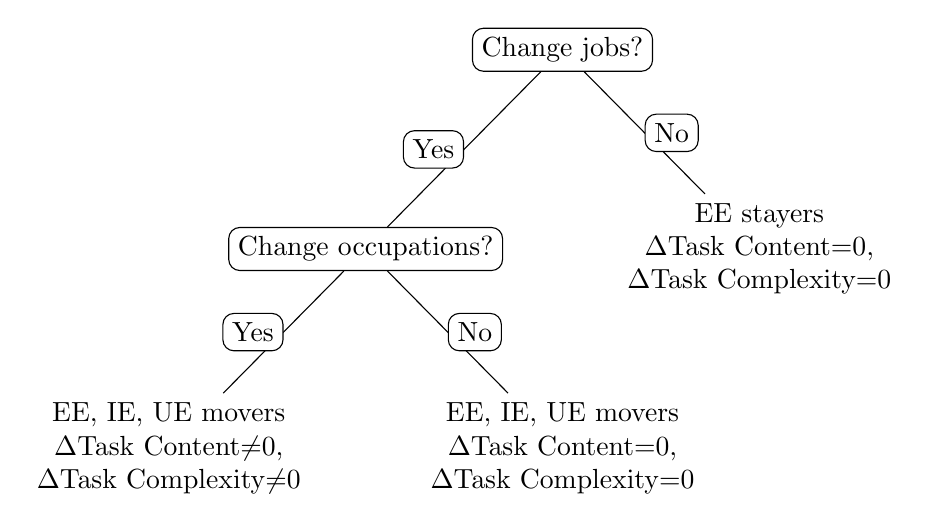
\begin{tikzpicture}[sibling distance=5cm,
			every node/.style = {shape=rectangle, rounded corners,
				draw, align=center,
				top color=white}]]
			\tikzset{level distance=72pt}
			\node {Change jobs?}
			child {node {Change occupations?} child {node[draw=none,fill=none]{EE, IE, UE movers\\$\Delta$Task Content$\neq$0, \\ $\Delta$Task Complexity$\neq$0} edge from parent node[left] {Yes}} child {node[draw=none,fill=none]{EE, IE, UE movers \\ $\Delta$Task Content=0, \\ $\Delta$Task Complexity=0} edge from parent node[right] {No}} edge from parent node[left] {Yes}}
			child {node[draw=none,fill=none]{EE stayers \\ $\Delta$Task Content=0, \\ $\Delta$Task Complexity=0} edge from parent node[right] {No}};
		\end{tikzpicture}
		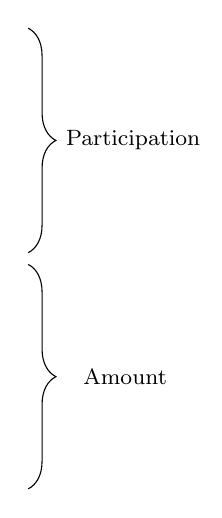
\begin{tikzpicture}
			\draw [decorate,decoration={brace,amplitude=10pt},xshift=-4pt,yshift=0pt] (3.5,7.5) -- (3.5,4.65) node [black,midway,xshift=35pt,text width=1.5cm] {\footnotesize  Participation};
			\draw [decorate,decoration={brace,amplitude=10pt},xshift=-4pt,yshift=0pt] (3.5,4.5) -- (3.5,1.65) node [black,midway,xshift=35pt] {\footnotesize Amount};
		\end{tikzpicture}
	\end{center}
	\caption{Illustration of Double Hurdle model} \label{fig:flowE2E}
	\caption*{\footnotesize{Notes: In labour market transitions, either an an individual changes jobs or stays in their current position. If an individual changes jobs they may also change occupations and therefore have a task content or task complexity change}}
\end{figure}
		
\noindent Our empirical specification must capture the two-step nature of the decision to change tasks, as illustrated in figure \ref{fig:flowE2E}. The first step participation decision is whether or not to change jobs between the first and second quarters of an individual transition. Importantly, this step typically incurs fixed costs. Therefore a Tobit specification - which would assume a single mechanism to drive both the participation and amount decision - is inappropriate. A familiar modelling approach in such two-step problems is the Heckit model advanced by \cite{Heckman}. However, this model assumes first hurdle dominance - ie. that in the second stage there will be no zero observations. This is not appropriate in the current setting as a zero task content/complexity move is a valid choice, shown by those who change jobs but do not move occupations in figure \ref{fig:flowE2E}, and represents approximately 40\% of all job changers. This motivates our choice of a Double Hurdle specification, proposed by \cite{cragg1971}, and applied in a labour market setting by \cite{BlundellMeghir} and \cite{Blundell1989}. This model captures both the extensive (participation decision) and intensive (amount decision) of task content and task complexity change during employment transitions and allows them to be governed by distinct stochastic processes. It also allows the outcome variable to take the value of zero in the second stage.
Concretely, the equations of the Double Hurdle model are:

	\begin{subequations}
	\label{eqn:heckman}
	\begin{align}
		& d^{*}_{it,2} = \tilde{\alpha}_0 + \tilde{\alpha}_{1}u_{t,2}  + \sum_{j} \tilde{\beta}_{j}\hat{X}_{j,it,1} + \sum_{k} \tilde{\gamma}_{k} \text{Q}_{k,2} + \sum_{l} \tilde{\delta}_{l} \text{R}_{l,1} + \sum_{m} \tilde{\zeta}_{m} \text{I}_{m,1} +  \tilde{\epsilon}_{it} \label{eqn:a}\\
		& y_{it,2}^{**} = \check{\alpha}_0 + \check{\alpha}_{1}u_{t,2} + \sum_{j} \check{\beta}_{j}X_{j,it,12} + \sum_{k}\check{\gamma}_{k} \text{Q}_{k,2} + \sum_{l} \check{\delta}_{l} \text{R}_{l,1}  + \sum_{m} \check{\zeta}_{m} \text{I}_{m,1} + \hat{\lambda}_{it} + \check{\epsilon}_{it} \label{eqn:b} \\
		& d_{it,2} =
		\begin{cases}
			1, & \text{if}\  d^{*}_{it,2} >0  \\
			0, & \text{if}\ d^{*}_{it,2} \leq0  
		\end{cases}\label{eqn:c}\\
		& y_{it,2}^* =\max(0, y_{it,2}^{**})  \label{eqn:d} \\
		& y_{it,2} = d_{it,2}\; y_{it,2}^* \label{eqn:e} 
	\end{align}
\end{subequations}

Where subscripts refer to individual $i$, subscripts $_1$, $_2$ and $_{12}$ refer to data in the first quarter, second quarter, and both quarters of a transition at time $t$, respectively. $Q$ are quarter, $R$ region and $I$ industry fixed effects; $\tilde{\epsilon}_{it}$ and $\check{\epsilon}_{it}$ are error terms. Equations \ref{eqn:a} and \ref{eqn:b} represent the participation and amount hurdles, respectively.  $\hat{X}$ and $X$ are a set of controls which include demographic characteristics, namely age and age squared, marital status, sex, level of education,\footnote{We split education into low, medium and high. In the low category we only include individuals with no qualifications; in the middle we include those with at least an Entry Level Qualification and at most A levels (a UK pre-requisite for university entry); and in the high we include all those with any qualification above A levels.} number of children. We also add a set of variables related to the individual's current and previous job: the duration of the previous employment and whether the separation was voluntary/involuntary or related to retirement, as well as controls for whether either job is temporary, part- or full-time, self-employed, and in the public or private sector. Finally, we have a set of controls for the method by which the individual searches for new jobs: through a job centre, ads, direct applications, family/friends, or some other method.  Note that control variables in the participation equation, $\hat{X}$, differ from those in the amount equation, $X$, in \ref{eqn:b}. This is because this hurdle uses the full estimation sample, which includes those who do not change jobs. As such, we only include controls for the first-period job (or, as we will use interchangeably, `previous' job.) For the same reason we also omit search method and separation type. Finally, $\hat{X}$ also includes an exclusion restriction, which we discuss below. The independent variable of interest is the aggregate unemployment rate, $u_{t,2}$.  $\hat{\lambda}$ is the estimated inverse Mills ratio obtained from estimating equation \ref{eqn:a}. 


\vspace{2mm}


Equation \ref{eqn:a} is the participation hurdle which captures desired task content or complexity move  $d^{*}$, which is latent. Equation \ref{eqn:b} and  \ref{eqn:d} are the amount hurdle, which is a Tobit model. In equation \ref{eqn:e}, $y_{it,2}$ describes the data actually observed, which captures the combined effect of the participation decision (equations \ref{eqn:a}, \ref{eqn:c}) and the amount decision (equation \ref{eqn:b} and \ref{eqn:d}). $y_{it,2}$ is either $\Delta\text{\textit{Task Content}}_{it,2}$ 
or $|\Delta\text{\textit{Task Complexity}}_{it,2}|$. For the latter we take the absolute value of the change in task complexity since we cannot have an upper and lower truncation limit for the Tobit equal to zero as this would imply no truncated values. 

\vspace{2mm}

We allow for correlation in the error terms of the first and second hurdles, since table \ref{tab:diffMeans} suggests there are significant differences in observable characteristics between the recession and and non-recession samples. Those that transition in a recession are older, more likely to be married, and have longer tenure. Fewer are in temporary roles for their previous job, and a larger fraction are self employed or work for the public sector in either their previous or current job. Fewer are medium-educated and a higher fraction are low- educated. More have quit (made a voluntary separation) from their previous employer, and a smaller fraction have been fired (made an involuntary separation).  It is likely, therefore, that there are unobserved factors that affect the participation decision and also affect the amount decision.



%\vspace{2mm}


%The Double Hurdle model has the advantage of allowing the extensive (participation) and intensive (amount) margins to be governed by distinct stochastic processes. That is, unlike a simple Tobit model, it allows different processes to determine the value of the continuous (non-zero) observations and the discrete switch at zero. This is important for our purposes since there is no reason to expect that the relationship between the unemployment rate and the extensive margin (the decision to change task content/complexity) to be the same as the intensive margin (the amount to change task content/complexity) due to the presence of fixed costs incurred during the participation decision. This modelling approach is also related to the control function advanced by \cite{Heckman}, but whereas the Heckit model assumes first hurdle dominance, i.e. that in the second stage there will be no zero observations, the Double Hurdle model allows zero observations to arise, important in this case as a zero task content/complexity move is a valid choice. As in a Heckman model, we allow the errors of the first and second hurdles to be correlated.

\vspace{2mm}

To identify the effect of the first hurdle we include the exclusion restriction \textit{Wait}, whether the individual is waiting to start a job that they have already obtained. The exclusion restriction for the selection equation is a dummy which captures whether an individual is waiting to start working in a job that they have already obtained. This applies to all flow types: EE, IE and UE. It captures those still employed but that have obtained a new job (EE). It also covers those who are inactive as they are not currently employed and not seeking work but are waiting to take up a position (IE). Finally, those unemployed and waiting to take up a position (UE) are distinguished from those who are inactive as they have been actively seeking employment in the last 4 weeks. It is also highly but not perfectly predictive of the dependent variable in the selection equation - whether the individual changed jobs between the first and second quarter of their survey - since many people that are waiting to take up a job will change jobs within the survey window, as table \ref{tab:t_test_jobMove_ALL} in the appendix demonstrates. However, it is not related to the size of the task content or complexity change that an individual makes upon changing jobs conditional on transition type, as a difference in mean task move between those who waited to take up a position and those that didn't (\ref{tab:t_test_wait_EE} - \ref{tab:t_test_wait_UE}, appendix) confirms.


	\newpage
\thispagestyle{empty}
\begin{table}[H]
	\centering
	\caption{Difference in Means Of Observable Characteristics}\label{tab:diffMeans}
	\begin{adjustbox}{max width=16cm, max height=10cm}
		\begin{threeparttable}
			\input{../Results/t_test_temp.tex}
			\begin{tablenotes}
				\item \footnotesize{Notes: Difference in longitudinal-weighted means when the aggregate unemployment rate is above=1 and below=0 the unemployment rate average for all transitions resulting in a job move in the synthetic 2Q sample. Significance levels:$ \quad ^{*}<10\% \quad ^{**}<5\% \quad ^{***}<1\%$. Standard errors in parentheses. Source: author's calculations.}  
			\end{tablenotes}
		\end{threeparttable}
	\end{adjustbox}
\end{table}


	\section{Results}
	\label{sec:results}
	
	
Table \ref{tab:TobitResults} details the estimation results of equations \ref{eqn:heckman}. Columns 2 - 7 show the results with with dependent variable $\Delta$ Task Content. `ALL', `EE' and `IE \& UE' headings refer to the sample used in the estimation which depends on labour market transition type. 'Above' and 'Hurdle' refer to the participation and amounts equations, respectively.


 For all transition types (EE and IE/UE) , we see an increase in the aggregate unemployment rate is associated with an increase in the likelihood of changing tasks content by 0.23 standard deviations.
	
		\newpage
	\newgeometry{a4paper,left=1in,right=1in,top=1in,bottom=1in,nohead}
	%\begin{landscape}
	\thispagestyle{empty}
	\begin{table}[htbp]
		\centering
		\caption{Double-Hurdle Regression Output}\label{tab:TobitResults}
		\begin{adjustbox}{width=\textwidth}
			\begin{threeparttable}
				% \input{../Results/tobit_ALL_2000s.tex}
				
				\input{../Results/dh_temp_ALL_28062022.tex}
				\begin{tablenotes}
					\item{\footnotesize{Double Hurdle at the 4-digit occupation category level. ALL refers to all labour market transitions, EE refers to direct job-to-job transitions, IE \& UE refers to employment transitions with between 1 and 3 quarters of unemployment and/or inactivity in between. The coefficient on age squared is multiplied by 1000. The reference category for education is Low Education; for Job Separation it is `No Separation';  for Job seeking method it is `Not Looking'. The regression includes quarter and regional fixed effects. Standard errors in parentheses.}}
				\end{tablenotes}
			\end{threeparttable}
		\end{adjustbox}
	\end{table}
	%\end{landscape}
	\restoregeometry % Restore the global document page margins

	
	
	\newpage
	\thispagestyle{empty}
	\begin{figure}
		\centering
		\begin{subfigure}[b]{1\textwidth}
			\includegraphics[width=1\linewidth]{../Figures/meanangSep_EE_IEUE.pdf}
			\caption{}
			\label{fig:Ng1} 
		\end{subfigure}
		
		\begin{subfigure}[b]{1\textwidth}
			\includegraphics[width=1\linewidth]{../Figures/meanmodOfMod_EE_IEUE.pdf}
			\caption{}
			\label{fig:Ng2}
		\end{subfigure}
				\begin{subfigure}[b]{1\textwidth}
			\includegraphics[width=1\linewidth]{../Figures/Aggre_Ur_pct_2q.pdf}
			\caption{}
			\label{fig:Ng3}
		\end{subfigure}
		\caption[Mean $\Delta$ Task Content and $\Delta$ Task Complexity by Transition Type]{Five quarter moving average of the (a) $\Delta$ Task Content and (b) $\Delta$ Task Complexity within-quarter for EE, IE transitions.(c) Aggregate Unemployment Rate.}
	\label{fig:TaskSkillsUR}
	\end{figure}


		\newpage
	\clearpage

	
	\section{Concluding Remarks}
	\label{sec:Conclusion}
	

	%We study the extent to which the occupational content of job transitions is sensitive to cyclical fluctuations. Using the UK Labour Force Survey matched with the O*NET dictionary of tasks for the period \input{../Results/min_date.txt}\hspace{-1mm}-\input{../Results/max_date.txt}\hspace{-1mm}, we find little evidence for an economically significant relationship. Unlike previous research, we focus on observed changes in the task content and task complexity of job transitions, not only on changes in occupational category. 
	
	
\begin{comment}
	
	Our first econometric specification sits closest to the existing literature; we use a Tobit model to estimate the relationship between business cycles and the propensity to make occupational changes. Novel to our paper is the addition of task content and complexity data. This captures not only the extensive margin of whether people make occupational transitions in recessions, but also the intensive margin of the extent of task content and complexity change. We find a relationship in the same direction as existing studies: task content and task complexity distances decrease in recessions. However the economic significance of the result is small, and by using a McDonald-Moffit decomposition we show that this is because the intensive margin of the extent of occupational change comprises over \input{../Results/fracMeanPos_angSep_CASCOT_r.txt}\hspace{-1mm}\% of the total relationship. Furthermore, we aggregate the task content and complexity data to the one-digit SOC code level, and show that our result is not simply a result of using more disaggregated data. These results, along with evidence of selection effects in the types of people that change jobs in a recession, suggests a need to capture both the decision to change employers and the decision to make an occupational change. Our final specification, which uses a Double Hurdle model, captures this two-stage decision process and allows for selection. We show that the estimates under this specification show an  insignificant relationship between recessions and the intensive margin of occupational change. In recessions, individuals make smaller occupational changes - but this is driven entirely by a slowing down in the rate of employer change, along with selection effects: the types of people that make employer changes in recessions also tend to make smaller occupational task content and task complexity moves.
	
	
	\end{comment}
	
	%% The Appendices part is started with the command \appendix;
	%% appendix sections are then done as normal sections
	%% \appendix
	
	%% \section{}
	%% \label{}
	
	%% If you have bibdatabase file and want bibtex to generate the
	%% bibitems, please use
	%%
	%%  \bibliographystyle{elsarticle-harv} 
	%%  \bibliography{<your bibdatabase>}
	
	%% else use the following coding to input the bibitems directly in the
	%% TeX file.
	
	
	
	%\begin{thebibliography}{00}
	
	%\bibliographystyle{elsarticle-harv} 
	%\bibliography{<your bibdatabase>}
	
	
	
	%\end{thebibliography}
	\newpage
	\section{Acknowledgements}
	
	An earlier version of this paper formed part of both authors' PhD theses, and as such would like to thank our supervisors Liang Bai, Mike Elsby, Maia G\"{u}ell, and Ludo Visschers for their guidance. We also thank Carlos Carrillo-Tudela, Cristina Lafuente, Eva Pocher, Jean-Marc Robin, Tuomas Pekkarinen, Anna Salomons, Mark Schaffer and Jonathan Thomas as well as participants from conferences at Economics at Panmure House, EEA-ESEM, EALE, ESPE, RES, SaM, SGPE, SMYE, SGPE; from seminars at Aalto University, The University of Edinburgh, ETLA,  IAB, Scottish Government and VATT. 
	\newpage
	\appendix
	\setcounter{table}{0}
	\section{Description of Regression Variables}
	\label{app:regVars}
	
		\resizebox{\textwidth}{!}{%
		\begin{tabular}{l*{1}{ll}}
			\hline\hline
			&        Name &          Description\\
			\hline
			&   Aggregate Unemployment Rate&  Aggregate unemployment rate, calculated using 2Q Quarterly LFS and ONS definitions\\
			&   Regional-Aggregate Unemployment Rate&   Regional minus aggregate unemployment rate\\
			& Female & Sex dummy, 1 = female 0 = male \\
			& Age & Age in years in first quarter of transition \\
			& Age$^2$ & Age squared \\
			& Married/Cohabitating & Dummy, 1=Married/Cohabitating \\
			& Number of Children & Number of children in household  \\
			& High Education & Education above university entry-level (above A-level, Highers or IB) \\
			& Medium Education & Education up to university entry-level \\
			& Low Education & No Qualifications \\
			& Previous Employment Duration & Time spent at previous job according to LFS definition: \\
			& & 1 = less than 3 months, 2 = 3-6 months, 3 = 6-12 months, 4 = 1-2 years, \\
			& & 5 = 2-3 years, 6 = 3-4 years, 7 =4-5 years, 8 = 5+ years\\
			& Full time, previous job & Dummy, 1 = full time in previous job\\
			& Full time, current job & Dummy, 1 = full time in current job\\
			& Public sector, previous job & Dummy, 1 = public sector in previous job\\
			& Public sector, current job & Dummy, 1 = public sector in current job\\
			& Self-employed, previous job & Dummy, 1 = self-employed in previous job\\
			& Self-employed, current job & Dummy, 1 = self-employed in current job\\
			& Looking for job & Dummy, 1 = was looking for job in first quarter \\
			& Job Mover & Dummy, 1 = moved jobs  \\
			& Separation: Involuntary & Dummy, 1 = fired or made redundant \\
			& Separation: Voluntary & Dummy, 1 = quit  \\
			& Separation: Other & Dummy, 1 = retired, health issues, other\\
			& Method of seeking: Agency & Dummy, 1 = got job through employment agency (reference category)\\
			& Method of seeking: Job Centre & Dummy, 1 = got work through job centre\\
			& Method of seeking: Ad& Dummy, 1 = got work through applying to advertisement\\
			& Method of seeking: Direct Application & Dummy, 1 = direct application to employer\\
			& Method of seeking: Family/Friend & Dummy, 1 = through family/friends \\
			& Method of seeking: Other & Dummy, 1 = other method\\
			& Wait & Dummy, 1 = waiting to take up job already obtained \\
			& Quarters & Quarters, 1-4 \\
			& Regions & Regions of the UK according to LFS definitions, 1-20 \\
			\hline
			\hline\hline
		\end{tabular}}


	
	\newpage
	\section{Summary Statistics}
	\label{app:SummaryStats}
	
	
	% Table A1: Summary statistics for SOC 2010-O*NET matches
	\input{../Results/SOC_ONETmatchDist.tex} 
	
	% Table A2: Number of Job Movers (ALL transitions)
	%\input{../Results/jobMoverTab.tex} 
	%\vspace{2mm}
	
		% Table A2: Number of Job Movers (by transition type)
		\input{../Results/jobMoverTabbyStatus.tex} 
			\vspace{2mm}
	
	% Table A3: Mean and sd of change in tasks and skills by job move
	% can change tasks & skills without changing employer
	\input{../Results/angSepJobMove.tex} 
		\vspace{2mm}
	
	% Table A4: Number of  tasks and skills movers by transition type
	\input{../Results/angSepTabbyStatus.tex} 
	\vspace{2mm}
	
		% Table A4: Mean and sd of change in tasks and skills by task/skill move (lower than table above as approx 50% of those who move jobs also move skills.
	\input{../Results/angSepTaskMove.tex} 
	
	\vspace{2mm}
	% Table A5 : Mean and sd of job mover by task/skill move
	\input{../Results/angSepjobMover.tex} 
	
	
	\vspace{2mm}
	% Table A6 : Mean and sd of independent variables by job move
	\input{../Results/regVars_jobMove.tex} 
	
	\vspace{2mm}
	% Table A7: Mean and sd of independent variables by transition type, all job movers 
	\input{../Results/regVars_statusJobMove.tex} 
	
	\vspace{2mm}
	
	%\input{../Results/regVars_statusJobStay.tex} 
	
	\vspace{2mm}
	
	
	\input{../Results/t_test_wait_EE.tex} 
		\input{../Results/t_test_wait_IE.tex} 
			\input{../Results/t_test_wait_UE.tex} 
	\vspace{2mm}
	
	\input{../Results/t_test_jobMove_ALL.tex} 
	
	\vspace{2mm}
	
	%\input{../Results/waitTaskMove.tex} 
	\newpage
		\section{Robustness Checks}
	%	\setcounter{equation}{0}
	\label{app:Robust}
	
	
		\subsection{Two-Task Example of the Task Content and Complexity Change Measures}
	\label{sec:twoTaskEx}
	
		Figure \ref{fig:AngSep} provides an illustration of how the $\Delta$Task Content and $\Delta$Task Complexity measures can provide us with information about the content of occupational moves. We construct a basic example in which there are a total of four different occupations ($A$, $B$, $C$, $D$) which comprise two tasks: task 1 and task 2. Moving from occupation $A$, which has a high level of complexity in task 1 and task 2, to $B$, which has a low level of complexity in both tasks gives a change in task content of 0, since the tasks are still used in the same proportion. The $\Delta$Task Complexity$_{o,o'}$ of $\input{../Figures/AB_skillScore.txt}$ reflects the fact that occupation $B$ is much lower skilled than $A$. Moving from occupation $C$ to $A$ represents both a change in task content and increased complexity, whereas the change in tasks from $A$ to $D$ constitutes reduced complexity. Finally, moving from and to the same occupation $A$ results in zeros for both measures.
	
	\begin{figure}[H]
		\centering
		\includegraphics[scale=0.50]{../Figures/AngularSeparation_example}
		\qquad
		\begin{tabular}{lcc}
			& $\Delta$Task Content$ _{o,o'}$& $\Delta$Task Complexity$_{o,o'}$\\
			\hline
			\hline
			A $\rightarrow$ B & 0 & \input{../Figures/AB_skillScore.txt}  \\
			C $\rightarrow$ A &  \input{../Figures/CA_angSep.txt} & \input{../Figures/CA_skillScore.txt}  \\
			A $\rightarrow$ D &  \input{../Figures/AD_angSep.txt} & \input{../Figures/AD_skillScore.txt}  \\
			A $\rightarrow$ A & 0 & 0 \\
		\end{tabular}
		\caption{An example of $\Delta$Task Content  and $\Delta$Task Complexity with 2 tasks and 4 occupations}
		\caption*{\footnotesize{Notes: In this example, there are two tasks, task 1 and 2 and 4 occupations, A, B, C and D with differing task content (the angle of the vector) and task complexity intensities (the magnitude of the vector). The tables report calculated $\Delta$ Task Content and $\Delta$ Task Complexity for reported occupation pairs.}}
		\label{fig:AngSep}
	\end{figure}
	

	
	
	
		\subsection{The Relationship between Task Complexity and Wages}
	\label{sec:wagesSkills}
	In using the $\Delta$Task Complexity measure, equation \ref{eq:skillScore}, we are assuming that vector length of occupations is a good proxy for complexity or skill requirement of the tasks completed in an occupation. If the measure is capturing this we should expect it to be positively correlated with wages. To test this assumption we calculate the task complexity level for each occupation in the LFS: \\
	
	Task Complexity Level$_{o}$ = $\left[\sum_{t=1}^{T}(q_{t,o}^{2})\right]^{\frac{1}{2}} $ \\
	
	\noindent  i.e. it is a measure of the vector length of an occupation in the task space, or the left hand side of the term in brackets of equation \ref{eq:skillScore}. We use this measure in a standard Mincerian wage estimation: 
	\begin{equation}
		\label{eq:skill_returns}
		\ln w_{it}= \alpha + \beta_{1}\text{Task Complexity Level}_{o}+  \sum_{k} \beta_{k}X_{k,it} + e_{it}, 
	\end{equation}
	
	where $\ln w_{it}$ are log real gross weekly wages for individual $i$ at time $t$. The vector $X_{it}$ includes controls for age, age squared, a dummy equal to 1 for female, years of tenure in the current job and dummies for high, medium and low eduction. Task Complexity Level is standardised by subtracting its mean and dividing by its standard deviation to facilitate interpretation. We use the five quarter LFS which records wage in the first and fifth quarter of interview, we take the wage to be the one seen in the last quarter of interview. The sample includes all types of job histories ending with employment in the fifth quarter of interview.
	
	\vspace{2mm}
	
	The estimation of Equation \ref{eq:skill_returns} can been seen in table \ref{skill_returns}. A one standard deviation increase in task complexity level is associated with an increase of \input{../Results/beta_SkillTotal.txt}\hspace{-1mm}\% in weekly gross real wages. This result suggests that our measure of the length of the vector as a task complexity proxy is reasonable since it is strongly positively correlated with wages. 
	
	
	\begin{table}[t]
		\centering
		\begin{tabular}{l*{1}{c}}
			\input{../Results/returns_skill_2000s}
		\end{tabular}
		\caption{Estimated Returns to Task Complexity} 
		\caption*{\footnotesize Notes: Dependent variable is log real gross weekly wages. Estimated on the LFS 5Q sample of full time workers using wages observed in the first interview quarter for years 2000-2010. Task Complexity Level is proxied by linked O*NET data and standardised. The coefficient on Age$^2$ is multiplied by 1000. The reference category for education is Low Education (no qualifications). Standard errors in parentheses;	* \(p<0.10\), ** \(p<0.05\), *** \(p<0.01\)}
		\label{skill_returns}
	\end{table}
	
	

	
	
	
		\newpage
	\newgeometry{a4paper,left=1in,right=1in,top=1in,bottom=1in,nohead}
	%\begin{landscape}
	\thispagestyle{empty}
	\begin{table}[htbp]
		\centering
		\caption{Changes in Task Content and Task Complexity over the Cycle}\label{tab:ProbitResults}
		\begin{adjustbox}{width=0.5\textwidth}
			\begin{threeparttable}
				% \input{../Results/tobit_ALL_2000s.tex}
				
				\input{../Results/probit_temp_ALL.tex}
				\begin{tablenotes}
					\item{\footnotesize{(1) Tobit at the 4-digit occupation category level. (2) Tobit at the aggregated 1-digit occupation category level (3) Double Hurdle at the 4-digit occupation category level. The sample in the selection equation of specification (3) is all individuals aged 16-64 years old over the period \input{../Results/min_date.txt}\hspace{-1mm}-\input{../Results/max_date.txt}\hspace{-1mm} and employed in both the first and second quarter of their survey. The sample in all other other specifications have the additional restriction that individuals undertook a job transition over two quarters (i.e., changed employers). The coefficient on age squared is multiplied by 1000. The reference category for education is Low Education; for Job Separation it is `Voluntary';  for Job seeking method it is `Not Looking'. The regression includes seasonal, regional and industry fixed effects. Coefficients should be  multiplied by the APE factor where given to obtain correct marginal effect. Standard errors in parentheses.}}
				\end{tablenotes}
			\end{threeparttable}
		\end{adjustbox}
	\end{table}
	%\end{landscape}
	\restoregeometry % Restore the global document page margins
	\newpage
	
	\begin{comment}
	
	\clearpage
	
	\section{ Marginal Effects  and Decomposition of the Tobit Model}
	%	\setcounter{equation}{0}
	\label{app:TobitDecomp}
	
	\subsection{ Marginal Effects}
	The Tobit model can be expressed as:
	
	\begin{equation*}
	y_i= 
	\begin{cases}
	X_i \beta  + u_i ,& \text{if } \quad X_i \beta  + u_i >0\\
	0,              & \text{otherwise}
	\end{cases}
	\end{equation*}
	
	where $i=1,2,...,N$ with $N$ the number of observations, $y_i$ is the dependent variable. $X$ is a vector of independent variables, $\beta$ is a vector of coefficients and $u \sim N(0,\sigma^2)$ is the error term. 
	
	Unlike in an OLS regression, the marginal effect in equation \ref{eqn:tobit} of the main text has to be separately calculated. While in an OLS regression the marginal effect is simply $\frac{\partial E(y|X)}{\partial X_{j}}=\beta_j$, in Tobit the marginal effect can be written as follows:
	
	\begin{equation}
	\label{eqn:tobit_marginal}
	\frac{\partial E(y| X)}{\partial X_j} = P(y>0|X) \beta_j
	\end{equation}
	
	
	\noindent To get an estimate of the marginal effect, we assume a standard normal distribution of the data and we maximise the log-likelihood function of the tobit model w.r.t $\beta$ and $\sigma^2$. This will yield maximum likelihood estimates and, assuming that we have specified the model correctly, it will give us consistent and asymptotically efficient estimators for both $\beta$ and $\sigma^2$. We can then use $\hat{\beta}$ and $\hat{\sigma}$ to estimate the function $P(y>0|X)$. Using the appropriate expression for the standard normal distribution, we obtain $\hat{P}(y>0|X)=\frac{1}{N} \sum_{i=1}^N F(X_i \hat{\boldsymbol{\beta}}/ \hat{\sigma})$, where $F(.)$ is the CDF of a standard normal and N are the number of observations. Thus the marginal effect at the average is estimated as:
	\[
	\frac{\partial \widehat{E(y|X)}}{\partial X_j} = \underbrace{\frac{1}{N} \sum_{i=1}^N F(X_{i} \hat{\beta}/ \hat{\sigma})}_\text{APE scale factor} \hat \beta_j
	\]
	
	\noindent 
	Thus, for the purpose of interpretation of marginal effects, all coefficients that appear in the regression tables have to be multiplied by the APE scale factor to obtain the estimated marginal effect. 
	\vspace{3mm}
	
	\subsection{Decomposition of the Tobit Model}
	
	\noindent \cite{Tobin1958} shows that for the Tobit model the expected value of y is:
	\begin{eqnarray}
	E(y| X) = X \beta F(z) + \sigma f(z)
	\label{eqn:Ey}
	\end{eqnarray}
	
	
	where $z=X \beta/ \sigma$, $f(z)$ is the unit normal density and $F(z)$ is the corresponding CDF.
	
	\vspace{3mm}
	
	\noindent Furthermore, the expected value of y for observations above the limit, $y>0$, is $X \beta$ plus the expected value of the truncated normal error term (see \cite{Amemiya1973}):
	
	
	\begin{eqnarray}
	E(y|X, y>0)&=& E(y| X,u>-X \beta)\nonumber \\
	&=& X\beta + \sigma \frac{f(z)}{F(z)} \label{eqn:Ey*}
	\end{eqnarray}
	
	
	From \ref{eqn:Ey} and \ref{eqn:Ey*}, the relationship between $E(y|X)$ and $E(y|X,y>0)$ is simply:
	\begin{equation}
	E(y|X) = F(z)E(y|X, y>0)
	\label{eqn:eyey*rel}
	\end{equation}
	
	
	From \ref{eqn:Ey*}, taking the partial derivative with respect to the $jth$ independent variable  $X_j$ and noting that $F'(z) =  f(z)$ and $f'(z) = -zf(z)$ gives: 
	
	\begin{equation}
	\frac{\partial E(y|X,y>0)}{\partial X_j} = (1-zf(z)/F(z) - f(z)^2/F(z)^2)*\beta_j
	\label{eqn:EystarbyXi}
	\end{equation}
	
	
	\noindent From which $(1-zf(z)/F(z) - f(z)^2/F(z)^2)$ gives the fraction of the mean total response is due to the response above the limit, equation \ref{eqn:fracMeanResponse} in the main text.
	Taking the partial derivative of \ref{eqn:eyey*rel} with respect to $X_j$ gives: 
	
	\begin{equation}
	\frac{\partial E(y|X)}{\partial X_j} = F(z)\frac{\partial E(y|X,y>0)}{\partial X_j} +  E(y|X, y>0)\frac{\partial F(z)}{\partial X_j} 
	\label{eqn:MMdecomp}
	\end{equation}
	
	which, using the fact that $F(z) = P(y>0|X)$ and $\partial{F(z)}/\partial{X_j} = (\beta_j/\sigma)F(z)$  we can re-write as equation \ref{eqn:tobit_marginal}.
	Plugging \ref{eqn:EystarbyXi} into \ref{eqn:MMdecomp} gives the marginal effect for the Tobit:
	\begin{equation}
	\frac{\partial E(y|X)}{\partial X_j} = \frac{1}{N} \sum_{i=1}^N F(X\beta/ \sigma) \beta_j 
	\label{eqn:marginalTobit}
	\end{equation}
	
	
	\noindent Following \cite{Mcdonald1980}, using the estimates of $\beta$ and $\sigma$ we can get estimates for all parts of the decomposition in equation \ref{eqn:MMdecomp} at the average by recovering the corresponding $z$:
	
	\begin{align*}
	\label{eqn:decomposition}
	& F(z)\hat{\beta}_j = \frac{\partial E(y|X)}{\partial X_j} = \frac{1}{N} \sum_{i=1}^N F(X_j \hat{\beta}/ \hat{\sigma})\hat \beta_j \\
	& z = F^{-1}(X_j \hat{\beta}/ \hat{\sigma}) \\
	\end{align*}
	
	\end{comment}

	\newpage
	\clearpage
	\bibliographystyle{elsarticle-harv}
	\bibliography{taskSkillsCycle}
	
	
\end{document}

\endinput
%%
%% End of file `elsarticle-template-harv.tex'.
